\documentclass[tikz,border=5pt]{standalone}
\usepackage{fontspec}
\setmainfont{Times New Roman}
\usepackage{unicode-math}
\setmathfont{Cambria Math}
\usetikzlibrary{shapes.geometric,positioning,fit,backgrounds,arrows.meta,calc}

\begin{document}
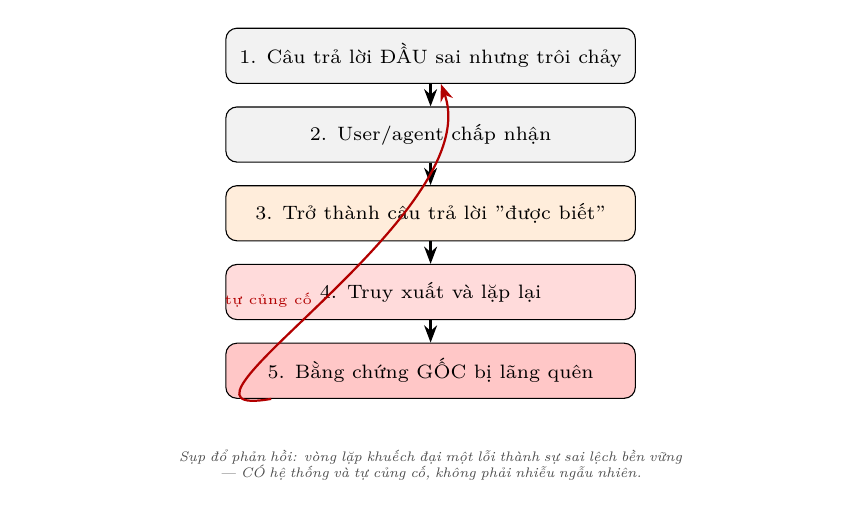
\begin{tikzpicture}[
  box/.style={rectangle, draw, rounded corners, align=center, font=\scriptsize, inner sep=3pt},
  arrow/.style={-{Stealth[length=2.2mm]}, thick},
  label/.style={font=\tiny\itshape, text=gray!60!black},
]

% === FEEDBACK COLLAPSE SEQUENCE ===
\node[box, fill=gray!10, minimum width=5.2cm, minimum height=0.7cm] (s1) at (0, 4.2) {1. Câu trả lời ĐẦU sai nhưng trôi chảy};
\node[box, fill=gray!10, minimum width=5.2cm, minimum height=0.7cm] (s2) at (0, 3.2) {2. User/agent chấp nhận};
\node[box, fill=orange!14, minimum width=5.2cm, minimum height=0.7cm] (s3) at (0, 2.2) {3. Trở thành câu trả lời "được biết"};
\node[box, fill=red!14, minimum width=5.2cm, minimum height=0.7cm] (s4) at (0, 1.2) {4. Truy xuất và lặp lại};
\node[box, fill=red!22, minimum width=5.2cm, minimum height=0.7cm] (s5) at (0, 0.2) {5. Bằng chứng GỐC bị lãng quên};

\draw[arrow] (s1) -- (s2);
\draw[arrow] (s2) -- (s3);
\draw[arrow] (s3) -- (s4);
\draw[arrow] (s4) -- (s5);
\draw[arrow, red!70!black] (s5) to[out=190,in=290] node[left, font=\tiny, text=red!70!black] {tự củng cố} (s1);

\node[label, align=center, text width=10cm] at (0, -1.0)
  {Sụp đổ phản hồi: vòng lặp khuếch đại một lỗi thành sự sai lệch bền vững\\— CÓ hệ thống và tự củng cố, không phải nhiễu ngẫu nhiên.};
\end{tikzpicture}
\end{document}